
%% bare_conf_compsoc.tex
%% V1.4b
%% 2015/08/26
%% by Michael Shell
%% See:
%% http://www.michaelshell.org/
%% for current contact information.
%%
%% This is a skeleton file demonstrating the use of IEEEtran.cls
%% (requires IEEEtran.cls version 1.8b or later) with an IEEE Computer
%% Society conference paper.
%%
%% Support sites:
%% http://www.michaelshell.org/tex/ieeetran/
%% http://www.ctan.org/pkg/ieeetran
%% and
%% http://www.ieee.org/

%%*************************************************************************
%% Legal Notice:
%% This code is offered as-is without any warranty either expressed or
%% implied; without even the implied warranty of MERCHANTABILITY or
%% FITNESS FOR A PARTICULAR PURPOSE! 
%% User assumes all risk.
%% In no event shall the IEEE or any contributor to this code be liable for
%% any damages or losses, including, but not limited to, incidental,
%% consequential, or any other damages, resulting from the use or misuse
%% of any information contained here.
%%
%% All comments are the opinions of their respective authors and are not
%% necessarily endorsed by the IEEE.
%%
%% This work is distributed under the LaTeX Project Public License (LPPL)
%% ( http://www.latex-project.org/ ) version 1.3, and may be freely used,
%% distributed and modified. A copy of the LPPL, version 1.3, is included
%% in the base LaTeX documentation of all distributions of LaTeX released
%% 2003/12/01 or later.
%% Retain all contribution notices and credits.
%% ** Modified files should be clearly indicated as such, including  **
%% ** renaming them and changing author support contact information. **
%%*************************************************************************


% *** Authors should verify (and, if needed, correct) their LaTeX system  ***
% *** with the testflow diagnostic prior to trusting their LaTeX platform ***
% *** with production work. The IEEE's font choices and paper sizes can   ***
% *** trigger bugs that do not appear when using other class files.       ***                          ***
% The testflow support page is at:
% http://www.michaelshell.org/tex/testflow/



\documentclass[conference,compsoc]{IEEEtran}
% Some/most Computer Society conferences require the compsoc mode option,
% but others may want the standard conference format.
%
% If IEEEtran.cls has not been installed into the LaTeX system files,
% manually specify the path to it like:
% \documentclass[conference,compsoc]{../sty/IEEEtran}





% Some very useful LaTeX packages include:
% (uncomment the ones you want to load)


% *** MISC UTILITY PACKAGES ***
%
%\usepackage{ifpdf}
% Heiko Oberdiek's ifpdf.sty is very useful if you need conditional
% compilation based on whether the output is pdf or dvi.
% usage:
% \ifpdf
%   % pdf code
% \else
%   % dvi code
% \fi
% The latest version of ifpdf.sty can be obtained from:
% http://www.ctan.org/pkg/ifpdf
% Also, note that IEEEtran.cls V1.7 and later provides a builtin
% \ifCLASSINFOpdf conditional that works the same way.
% When switching from latex to pdflatex and vice-versa, the compiler may
% have to be run twice to clear warning/error messages.






% *** CITATION PACKAGES ***
%
\ifCLASSOPTIONcompsoc
  % IEEE Computer Society needs nocompress option
  % requires cite.sty v4.0 or later (November 2003)
  \usepackage[nocompress]{cite}
\else
  % normal IEEE
  \usepackage{cite}
\fi
% cite.sty was written by Donald Arseneau
% V1.6 and later of IEEEtran pre-defines the format of the cite.sty package
% \cite{} output to follow that of the IEEE. Loading the cite package will
% result in citation numbers being automatically sorted and properly
% "compressed/ranged". e.g., [1], [9], [2], [7], [5], [6] without using
% cite.sty will become [1], [2], [5]--[7], [9] using cite.sty. cite.sty's
% \cite will automatically add leading space, if needed. Use cite.sty's
% noadjust option (cite.sty V3.8 and later) if you want to turn this off
% such as if a citation ever needs to be enclosed in parenthesis.
% cite.sty is already installed on most LaTeX systems. Be sure and use
% version 5.0 (2009-03-20) and later if using hyperref.sty.
% The latest version can be obtained at:
% http://www.ctan.org/pkg/cite
% The documentation is contained in the cite.sty file itself.
%
% Note that some packages require special options to format as the Computer
% Society requires. In particular, Computer Society  papers do not use
% compressed citation ranges as is done in typical IEEE papers
% (e.g., [1]-[4]). Instead, they list every citation separately in order
% (e.g., [1], [2], [3], [4]). To get the latter we need to load the cite
% package with the nocompress option which is supported by cite.sty v4.0
% and later.





% *** GRAPHICS RELATED PACKAGES ***
%
\ifCLASSINFOpdf
   \usepackage[pdftex]{graphicx}
  % declare the path(s) where your graphic files are
  % \graphicspath{{../pdf/}{../jpeg/}}
  % and their extensions so you won't have to specify these with
  % every instance of \includegraphics
  % \DeclareGraphicsExtensions{.pdf,.jpeg,.png}
\else
  % or other class option (dvipsone, dvipdf, if not using dvips). graphicx
  % will default to the driver specified in the system graphics.cfg if no
  % driver is specified.
  % \usepackage[dvips]{graphicx}
  % declare the path(s) where your graphic files are
  % \graphicspath{{../eps/}}
  % and their extensions so you won't have to specify these with
  % every instance of \includegraphics
  % \DeclareGraphicsExtensions{.eps}
\fi
% graphicx was written by David Carlisle and Sebastian Rahtz. It is
% required if you want graphics, photos, etc. graphicx.sty is already
% installed on most LaTeX systems. The latest version and documentation
% can be obtained at: 
% http://www.ctan.org/pkg/graphicx
% Another good source of documentation is "Using Imported Graphics in
% LaTeX2e" by Keith Reckdahl which can be found at:
% http://www.ctan.org/pkg/epslatex
%
% latex, and pdflatex in dvi mode, support graphics in encapsulated
% postscript (.eps) format. pdflatex in pdf mode supports graphics
% in .pdf, .jpeg, .png and .mps (metapost) formats. Users should ensure
% that all non-photo figures use a vector format (.eps, .pdf, .mps) and
% not a bitmapped formats (.jpeg, .png). The IEEE frowns on bitmapped formats
% which can result in "jaggedy"/blurry rendering of lines and letters as
% well as large increases in file sizes.
%
% You can find documentation about the pdfTeX application at:
% http://www.tug.org/applications/pdftex





% *** MATH PACKAGES ***
%
%\usepackage{amsmath}
% A popular package from the American Mathematical Society that provides
% many useful and powerful commands for dealing with mathematics.
%
% Note that the amsmath package sets \interdisplaylinepenalty to 10000
% thus preventing page breaks from occurring within multiline equations. Use:
%\interdisplaylinepenalty=2500
% after loading amsmath to restore such page breaks as IEEEtran.cls normally
% does. amsmath.sty is already installed on most LaTeX systems. The latest
% version and documentation can be obtained at:
% http://www.ctan.org/pkg/amsmath





% *** SPECIALIZED LIST PACKAGES ***
%
%\usepackage{algorithmic}
% algorithmic.sty was written by Peter Williams and Rogerio Brito.
% This package provides an algorithmic environment fo describing algorithms.
% You can use the algorithmic environment in-text or within a figure
% environment to provide for a floating algorithm. Do NOT use the algorithm
% floating environment provided by algorithm.sty (by the same authors) or
% algorithm2e.sty (by Christophe Fiorio) as the IEEE does not use dedicated
% algorithm float types and packages that provide these will not provide
% correct IEEE style captions. The latest version and documentation of
% algorithmic.sty can be obtained at:
% http://www.ctan.org/pkg/algorithms
% Also of interest may be the (relatively newer and more customizable)
% algorithmicx.sty package by Szasz Janos:
% http://www.ctan.org/pkg/algorithmicx




% *** ALIGNMENT PACKAGES ***
%
%\usepackage{array}
% Frank Mittelbach's and David Carlisle's array.sty patches and improves
% the standard LaTeX2e array and tabular environments to provide better
% appearance and additional user controls. As the default LaTeX2e table
% generation code is lacking to the point of almost being broken with
% respect to the quality of the end results, all users are strongly
% advised to use an enhanced (at the very least that provided by array.sty)
% set of table tools. array.sty is already installed on most systems. The
% latest version and documentation can be obtained at:
% http://www.ctan.org/pkg/array


% IEEEtran contains the IEEEeqnarray family of commands that can be used to
% generate multiline equations as well as matrices, tables, etc., of high
% quality.




% *** SUBFIGURE PACKAGES ***
%\ifCLASSOPTIONcompsoc
%  \usepackage[caption=false,font=footnotesize,labelfont=sf,textfont=sf]{subfig}
%\else
%  \usepackage[caption=false,font=footnotesize]{subfig}
%\fi
% subfig.sty, written by Steven Douglas Cochran, is the modern replacement
% for subfigure.sty, the latter of which is no longer maintained and is
% incompatible with some LaTeX packages including fixltx2e. However,
% subfig.sty requires and automatically loads Axel Sommerfeldt's caption.sty
% which will override IEEEtran.cls' handling of captions and this will result
% in non-IEEE style figure/table captions. To prevent this problem, be sure
% and invoke subfig.sty's "caption=false" package option (available since
% subfig.sty version 1.3, 2005/06/28) as this is will preserve IEEEtran.cls
% handling of captions.
% Note that the Computer Society format requires a sans serif font rather
% than the serif font used in traditional IEEE formatting and thus the need
% to invoke different subfig.sty package options depending on whether
% compsoc mode has been enabled.
%
% The latest version and documentation of subfig.sty can be obtained at:
% http://www.ctan.org/pkg/subfig




% *** FLOAT PACKAGES ***
%
%\usepackage{fixltx2e}
% fixltx2e, the successor to the earlier fix2col.sty, was written by
% Frank Mittelbach and David Carlisle. This package corrects a few problems
% in the LaTeX2e kernel, the most notable of which is that in current
% LaTeX2e releases, the ordering of single and double column floats is not
% guaranteed to be preserved. Thus, an unpatched LaTeX2e can allow a
% single column figure to be placed prior to an earlier double column
% figure.
% Be aware that LaTeX2e kernels dated 2015 and later have fixltx2e.sty's
% corrections already built into the system in which case a warning will
% be issued if an attempt is made to load fixltx2e.sty as it is no longer
% needed.
% The latest version and documentation can be found at:
% http://www.ctan.org/pkg/fixltx2e


% correct bad hyphenation here
\hyphenation{op-tical net-works semi-conduc-tor}
\usepackage{float}


\begin{document}
%
% paper title
% Titles are generally capitalized except for words such as a, an, and, as,
% at, but, by, for, in, nor, of, on, or, the, to and up, which are usually
% not capitalized unless they are the first or last word of the title.
% Linebreaks \\ can be used within to get better formatting as desired.
% Do not put math or special symbols in the title.
\title{Distributed Denial of Service(DDoS) and DHCP Masquerading\\ Attack Vectors for Software-Defined Networks}


% author names and affiliations
% use a multiple column layout for up to three different
% affiliations
\author{\IEEEauthorblockN{Dogukan Yalcin}
\IEEEauthorblockA{Middle East Technical University\\Computer Engineering Department\\
E-mail: e194246@metu.edu.tr\\
}
\and
\IEEEauthorblockN{Tugca Eker}
\IEEEauthorblockA{Middle East Technical University\\Computer Engineering Department\\
E-mail: e194201@metu.edu.tr}}



% make the title area
\maketitle

% As a general rule, do not put math, special symbols or citations
% in the abstract
\begin{abstract}
Software-Defined Network is a state of art technology that constructed over the idea of control and data plane separation in the network. While this property provides many advantages like flexibility, centralization of management and simplification it also results in some security challenges. This report presents application of two attack vectors on SDN by using mininet virtual network environment; DDoS and DHCP Masquerading.
\end{abstract}
% no keywords

\IEEEpeerreviewmaketitle



\section{Introduction}
% no \IEEEPARstart
Software-Defined Networking (SDN) is an emerging architecture that is dynamic, manageable, cost-effective, and adaptable, making it ideal for the high-bandwidth, dynamic nature of today’s applications\cite{OpenNetworking}. SDN separates the network forwarding and control functions so that the related engineers or administrators will be able to solve or update the network from a distance.

The aim of this work is to simulate some SDN Specific network attacks and show their potential impacts by working on two specific attack vector; Distributed Denial of Service(DDoS) and DHCP Masquerading.


\section{Attack Vector: Distributed Denial of Service (DDoS)}

Denial-of-Service (DoS) attacks flood networks with an high-traffic in order to overwhelm the target resources and make it unavailable for non-malicious users. It means that DoS attack aims breaking of the availability component of the CIA triad. If more than one sources are used by the attackers, it becomes "Distributed" and identified as DDoS. According to Kalkan, Gur and Alagoz considering its design pillars and characteristics, DDoS attacks are also intrinsically viable of Software Defined Networks \cite{8030502}. 

SDN allows the decoupling of data and control planes in network devices to centralize control features by limiting the passive capabilities of switches. Since the controller becomes central property, DDoS attacks can cause fatal problems on the network if the controller penetrated with high \& malicious traffic.

\subsection{Impact and Real-life Examples}
IoT (Internet of Things) devices become more popular day by day and they're increasing in number. In Aug 2016, IoT devices pose enormous security thread against the well-known security journalist Brian Kreb's web site and French Web Host company OVH (Mirai Botnet). Nearly 400.000 hijacked devices shows impressive peak of 620 Gbps traffic against targets which causes OVH to stop their services. \cite{MiraiBotnet}

Likewise Mirai Botnet attack, well-known DDoS attacks such as UDP, ICMP, TCP SYN flooding, NTP amplification, and ping of death are also viable in Software-Defined Networks.\\ 
\subsection{Design \& Implementation}

\begin{figure}[H]
\centering
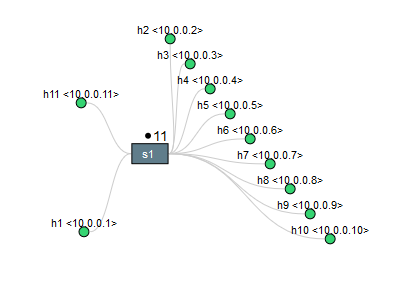
\includegraphics[width=0.5\textwidth]{ddos_schema.png}
\caption{\label{fig:diagram_1}Topology - Distributed Denial of Service.}
\end{figure}

Requirements:

\begin{itemize}
\item Floodlight
\item Sflow-RT
\item SimpleHTTPServer (Python)
\item hping3
\end{itemize}

\subsubsection{Topology}
As a network simulation environment we create a linear topology with 11 hosts, a single switch and a single controller. All hosts are directly connected to switch.  In our case, h1 is a web server and h11 is a non-malicious user which is always accessing to web server. All other hosts are (namely) IoT devices and they are members of the BotNET which is controlled by malicious attacker.


\subsubsection{Setup}
To initialize our network, we started by deploying HTTP Server on h1 node, which runs on port 80. To deploy server we used Python's SimpleHTTPServer library and created example index.html file as an example.

As a second step we configure the controller and the switch in our network. For the controller, we used OpenFlow - Floodlight. Also for tracing and monitoring the our network flow we setup a sFlow-RT instance in our environment and add our assets to it. After this step, we are able to manage and monitor our network via web interfaces of OpenFlow and sFlow. 



\subsection{Launching the Attack}


As a simulation of normal network traffic before the attack begins, the host h11 (non-malicious / non-attacker host), continuously requests the content of the index.html page and gets responses from the HTTP Server (host h1). \\

Launching the attack is done by using hping3 command with flood option to the HTTP server installed on h1. From h2 to h10 all hosts execute this command in order to make the HTTP server unable to respond other non-malicious requests. With each new execution of hping3 the HTTP server deals with increasingly more requests and higher network traffic. After a threshold, HTTP server cannot respond to any message from h11 (non-malicious) since it is busy with others' requests sent from h2-h10 which are unending. Hence h11 is unable to reach to the HTTP server. 

\subsection{Results \& Reasons of Success}
\begin{figure}[H]
\centering
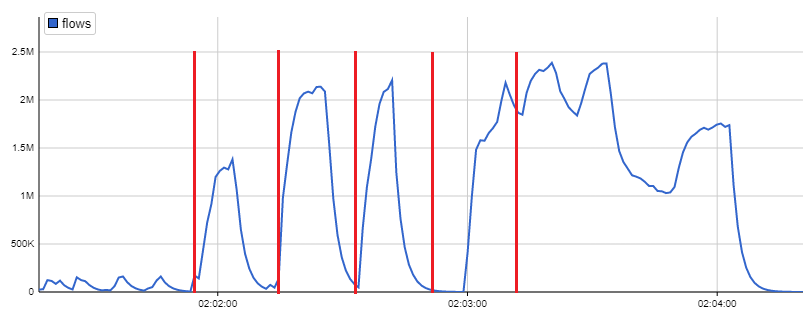
\includegraphics[width=0.5\textwidth]{attackers.png}
\caption{\label{fig:diagram_2}Graphic - Network Flow during DDoS Attack.}
\end{figure}

The figure above shows the flow-time relationship in the switch(s1). Initially only non-malicious user( h11 ) sends request to the server and gets related responses for 1 minute( until the first vertical red line in the figure ). Afterwards, malicious users started the attack one by one( at each vertical red line a new attacker is joined the attack ). The non-malicious user starts getting responses slower and slower with each new attacker. After the 4th attacker the server starts to struggle and eventually becomes unable to respond any requests. Starting from this time, the non-malicious user cannot get any response from the server.

The main reason for this attack's succession is the fact that for both data and control plane limited resources make SDN defenseless against the DDOS attacks. As a consequence, the connection between servers and end users can be blocked in SDNs by cause of the presence of  weak points in SDN architecture( Central Controller and separation of control planes ).

In conclusion, centralization of management feature of the SDN makes it vulnerable against DDoS attacks and attackers may target controller instruments on the network. This causes congestion on the network and non-malicious users may not be able to use network as they should. 

\subsection{Solutions \& Possible Future Work}
In order to deal with different sub-types of the DDoS Attack in Software-Defined Networks, there are several solutions in the literature. These solutions can be categorized as follows \cite{Kokila};

\begin{itemize}
\item Table-entry based solutions
\item Scheduling based solutions
\item Architectural solutions
\item Statistical Solutions
\item Machine Learning based solutions
\end{itemize}

If we focus on the Machine Learning based DDoS security solution; this mechanism trains itself with non-malicious / attack-free network packets and then classifies malicious network packets by machine learning algorithms. So, it gives detection ability to network; then different mitigation solutions can be applied on the network. As stated by Gopinat et al; dynamically scalable load balancers may be deployed and controlled by the SDN controller. \cite{DDosMitigation}

\section{Attack Vector: DHCP Masquerading}

Dynamic Host Configuration Protocol (DHCP) servers are utilized by network providers to provide Internet Protocol (IP) addresses, subnet masks, and gateway information. Hosts which are connected to network have an ability to pop-up rogue DHCP server which is not under the administrative control. Then they may become man-in-the-middle (MitM) and other users may be unaware of this malicious action. 

As non-malicious clients connect to network, rogue(masquerading) and legal DHCP servers will propagate the connection information packet which includes IP addresses, default gateway, DNS servers etc. If client accepts the packet which is created by rogue DHCP Server, it creates vulnerability that can be exploited by attacker if we assume that network doesn’t
have precautionary switches and local DNS cache servers.


\subsection{Impact and Sophistication}

Deploying a Rogue DHCP Server is an easy task for an attacker who already connected to the network. Clients may not have a chance to understand that there is a man-in-the-middle on the connection between themselves and the destination. Additionally, detecting \& stopping the Rogue DHCP server is not an easy task to do. Network needs intrusion detection system with appropriate signatures or multilayer switch structure to stop it. 

\subsection{Design \& Implementation}

\begin{figure}[H]
\centering
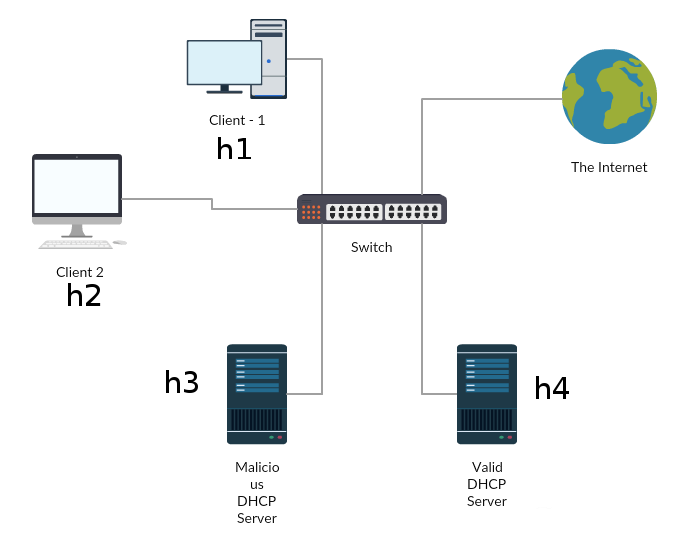
\includegraphics[width=0.5\textwidth]{dhcp_schema.png}
\caption{\label{fig:diagram_2}Topology - DHCP Masquerading.}
\end{figure}

\subsubsection{Topology}
As a network simulation environment we create a linear topology including 2 host, single good DHCP Server, single rouge (masquerading) DHCP server, single switch and single controller. Additionally in some way switch is connected to the Internet which allows hosts (Client-1, Client-2) to reach any web site like google.com or metu.edu.tr.  

To allow Malicious DHCP Server to respond earlier than good one, 500ms to 1s delay added to link between switch and the good DHCP Server (slower link). 

To sophisticate, attacker may add "Browser Mining Snippet" to the requested page's main page code and send it to victim as a response. Most probably, victim won't realize that a malicious entity is using it's system resources to mine cryptocoins.

\subsubsection{Setup}

After construction of the topology, we need to connect switch (s1) to the Internet. This is done by using mininet's NAT library. The library connects mininet topology to the Internet via NAT through eth0 on the host (mininet) machine. Then at this point, all hosts are able to connect to the Internet and request the content of the google.com or metu.edu.tr. 

Then; DHCP server deployed on the h4 which has slower connection rate, h1 or/and h2 also starts DHCP client using "dhclient" executable binary of the Linux. 

\subsection{Launching the Attack}

As a simulation of normal network traffic before the attack begins, the clients (h1 and h2) continuously requests web content. At some point attacker gets the control of the host h3 and does following;

 \begin{enumerate}
 \item Deploys malicious DHCP Server to masquerade the request coming from clients (udhcpd)
 \item Deploys fake DNS server to redirect clients to fake web-server (dnsmasq)
 \item Deploys web server to eavesdrop data communication, sniff or sending malicious  responses (Python SimpleHTTPServer)
 \end{enumerate}
 
After that, whenever clients make DHCP Request, request packet forwarded to both good DHCP server and malicious DHCP server. Since good DHCP server has a delayed connection; malicious DHCP server responds first and its response is accepted by the victim client. Malicious DHCP server provides its own network address as the DNS server address and deceives the victim. Then whenever victim make an DNS request (request to google.com initiates a DNS request call to get IP address of google.com), fake DNS server provides its own IP address instead of google.com's correct IP address. 

At this point, victim is connected to the malicious web server thinking it is connecting to google.com. So attacker may request victims credentials by imitating the design of google.com's main page or do whatever he/she want.

As stated on subsection 3.1, attacker may add "Browser Mining Snippet" to the Google's main page code and send it to victim as a response. Most probably, victim won't realize that a malicious entity is using it's system resources to mine cryptocoins and earn some "malicious" money.

\subsection{Solutions}

There are several methodologies to block attacker to successfully deploy rouge DHCP and become man-in-the-middle. Duangphasuk et al. suggest using digital  certificates to identify  the legal DHCP communication \cite{DHCPCertificate}. Also there is authentication based solution \cite{DHCPAuth}. But still these solutions makes hard the DHCP server or client implementation\cite{DHCPHard}.


Also, there is Software-Defined Network based defensive security solution which constantly monitors flows and resists against DHCP Rouge or DHCP Starvation attacks. It dynamically analyses all DHCP-related information on the packets using packet inspection. Then machine learning algorithm analyzes the data-set so it matches DHCP Server information, gateway and DNS information in the packet to avoid misconfiguration, roguing and any other malicious intention and informs DHCP clients about malicious entities.


\subsection{Reasons of Success \& Conclusion}

Dynamic Host Configuration Protocol (DHCP) is an automated mechanism to distribute IP addresses, gateways, DNS addresses and other network configuration information. By its nature, when DHCP clients propagates DHCP request; the first DHCP response received by host determines the network configuration which will be used by the host. This is the case for every single network system without exception if network does not have any additional security instrument. On this attack vector, we will make use of this commonality.

The fundamental ignorance is letting this attack to success which is the speed of the link(channel) between h4(the non-malicious DHCP Server) and the switch. The attacker observed the slowness of this link and used this information to become a man-in-the-middle with the help of a faster channel between his/her DHCP server and the switch.

\section{Conclusion}

In this report, we presented two different attack vector applications on SDN domain which is simulated on the Mininet Virtual Network. On DDoS attack vector example, we tried to show the idea of "Security for SDN" by explaining the vulnerabilities of the SDN against DDoS attacks. And for the DHCP Masquerading attack vector, we stated our arguments to explain "SDN for Security" idea.

% trigger a \newpage just before the given reference
% number - used to balance the columns on the last page
% adjust value as needed - may need to be readjusted if
% the document is modified later
%\IEEEtriggeratref{8}
% The "triggered" command can be changed if desired:
%\IEEEtriggercmd{\enlargethispage{-5in}}

% references section

% can use a bibliography generated by BibTeX as a .bbl file
% BibTeX documentation can be easily obtained at:
% http://mirror.ctan.org/biblio/bibtex/contrib/doc/
% The IEEEtran BibTeX style support page is at:
% http://www.michaelshell.org/tex/ieeetran/bibtex/
%\bibliographystyle{IEEEtran}
% argument is your BibTeX string definitions and bibliography database(s)
%\bibliography{IEEEabrv,../bib/paper}
%
% <OR> manually copy in the resultant .bbl file
% set second argument of \begin to the number of references
% (used to reserve space for the reference number labels box)
\begin{thebibliography}{1}

\bibitem{OpenNetworking}
Software-Defined Networking (SDN) Definition, {\em
What is SDN?} (2017), Retrived from https://www.opennetworking.org/sdn-definition/
\bibitem{8030502}
Kalkan, K., Gur, G., \& Alagoz, F. (2017). {\em
Defense Mechanisms against DDoS Attacks in SDN Environment.} IEEE Communications Magazine, 55(9), 175-179.
\bibitem{MiraiBotnet}
G. Kambourakis, C. Kolias and A. Stavrou, {\em
"The Mirai botnet and the IoT Zombie Armies"} MILCOM 2017 - 2017 IEEE Military Communications Conference (MILCOM), Baltimore, MD, USA, 2017, pp. 267-272.
\bibitem{floodlight}
Project Floodlight, {\em
Open Source Software for Building Software-Defined Networks}, http://www.projectfloodlight.org/floodlight/
\bibitem{Kokila}
R. Kokila et al., {\em
"DDoS Detection and Analysis in SDN-Based Environment Using Support Vector Machine Classifier"}, Proc. 2014 IEEE Sixth Int'l. Conf. Advanced Computing, pp. 205-10, 2014.
\bibitem{DDosMitigation}
Y, N., Gopinath, M., \& L, G. (2015). {\em
DDoS Mitigation using Software Defined Network.} International Journal of Engineering Trends and Technology, 24(5), 258-264. 

\bibitem{DHCPCertificate}
Duangphasuk, S., Kungpisdan, S., \& Hankla, S. (2011). Design and implementation of improved security protocols for DHCP using digital certificates. {\em2011 17th IEEE International Conference on Networks.}
\bibitem{DHCPAuth}
T. Aur \& M. Roe \& S. Murdoch, "Dynamic host configuration protocol"
U.S. Patent 8239549, Aug 7, 2012. 
\bibitem{DHCPHard}
Wang, J., \& Chen, Y. (2017). An SDN-based defensive solution against DHCP attacks in the virtualization environment. 2017 IEEE Conference on Dependable and Secure Computing. 
\end{thebibliography}




% that's all folks
\end{document}


